\documentclass[11pt]{article}
\usepackage[utf8]{inputenc}
\usepackage[T1]{fontenc}
\usepackage{amsmath}
\usepackage{amssymb}
\usepackage{multicol}
\usepackage{geometry}
\usepackage{tikz}
\usepackage{enumitem}
\usepackage{xcolor}
\usepackage{titlesec}

% Configurações de layout
\geometry{a4paper, left=1cm, right=1cm, top=0.5cm, bottom=1.2cm}
\setlength{\columnseprule}{0.4pt}

% Cores para títulos
\titleformat{\section}{\normalfont\Large\bfseries\color{blue}}{\thesection}{1em}{}
\titleformat{\subsection}{\normalfont\large\bfseries\color{red}}{\thesubsection}{1em}{}

\title{\textcolor{red}{Primeiro Trimestre: Matemática Financeira
    \\Juros Compostos}}
\author{Professor: Jefferson}
\date{}

\begin{document}

\maketitle
\vspace{-1cm}

%\begin{center}
%\large{Nome: \underline{\hspace{8cm}} \quad Turma: \underline{\hspace{3cm}}}
%\end{center}

\begin{multicols}{2}

\section*{Instruções}
    \textbf{Copie e responda no caderno e resolva os exercícios.}

\section*{Conceitos Básicos}

\subsection*{Capital (C)}
Valor inicial aplicado ou emprestado.

\subsection*{Taxa de Juros (i)}
Porcentagem cobrada pelo empréstimo ou ganha pelo investimento.

\subsection*{Tempo (t)}
Período da aplicação (em meses, anos, etc.).

\subsection*{Montante (M)}
Valor total ao final do período:
\[
M = C + J
\]
onde $J$ são os juros.

\section*{Juros Compostos - Fórmula Principal}

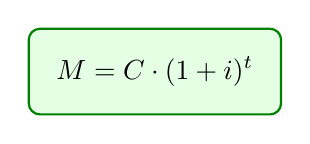
\begin{tikzpicture}
\node[rectangle, fill=green!10, rounded corners, inner sep=10pt, draw=green!50!black, thick] (box) {
$\displaystyle M = C \cdot (1 + i)^t$
};
\end{tikzpicture}

\subsection*{Fórmulas Derivadas}
\begin{itemize}
\item Montante: $M = C \cdot (1 + i)^t$
\item Juros: $J = M - C = C \cdot [(1 + i)^t - 1]$
\item Capital: $C = \dfrac{M}{(1 + i)^t}$
\item Taxa: $i = \sqrt[t]{\dfrac{M}{C}} - 1$
\item Tempo: $t = \dfrac{\ln\left(\frac{M}{C}\right)}{\ln(1 + i)}$
\end{itemize}

\subsection*{Características Fundamentais}
\begin{itemize}
\item \textbf{Crescimento exponencial} (progressão geométrica)
\item Juros sobre juros (juros capitalizados)
\item O juro é incorporado ao capital a cada período
\item Mais usado no mercado financeiro real
\item Ideal para períodos longos
\end{itemize}

\section*{Representação Gráfica}

\begin{center}
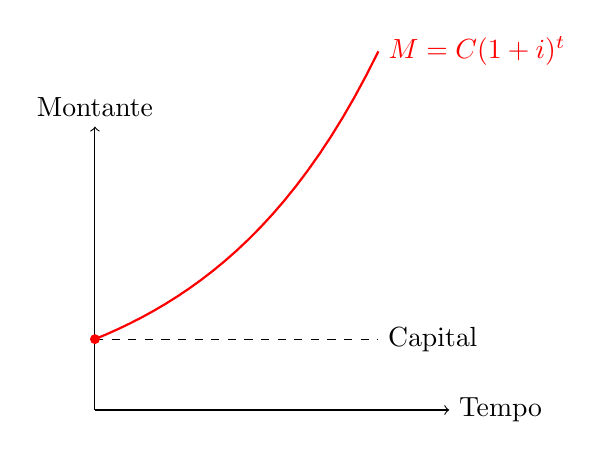
\begin{tikzpicture}[scale=0.9]
\draw[->] (0,0) -- (5,0) node[right] {Tempo};
\draw[->] (0,0) -- (0,4) node[above] {Montante};
\draw[red, thick, domain=0:4] plot (\x, {1.5^\x}) node[right] {$M = C(1 + i)^t$};
\draw[dashed] (0,1) -- (4,1) node[right] {Capital};
\fill[red] (0,1) circle (2pt);
\end{tikzpicture}
\end{center}

A função do montante é uma curva exponencial crescente.

\section*{Exercícios Básicos - Juros Compostos}

\begin{enumerate}[leftmargin=*]

\item Calcule o montante a juros compostos:
\begin{enumerate}[label=\alph*)]
\item $C = R\$ 1000$, $i = 2\%$ a.m., $t = 6$ meses
\item $C = R\$ 500$, $i = 1,5\%$ a.m., $t = 12$ meses
\item $C = R\$ 2000$, $i = 10\%$ a.a., $t = 2$ anos
\end{enumerate}

\item Calcule os juros compostos:
\begin{enumerate}[label=\alph*)]
\item $C = R\$ 1500$, $i = 2\%$ a.m., $t = 8$ meses
\item $C = R\$ 3000$, $i = 1\%$ a.m., $t = 1$ ano
\item $C = R\$ 5000$, $i = 12\%$ a.a., $t = 3$ anos
\end{enumerate}

\item Complete a tabela:
\begin{center}
\begin{tabular}{|c|c|c|c|}
\hline
\textbf{C} & \textbf{i} & \textbf{t} & \textbf{M (Compostos)} \\
\hline
R\$ 1000 & 2\% a.m. & 6 meses & \\
\hline
R\$ 500 & 12\% a.a. & 2 anos & \\
\hline
R\$ 2000 & 1,5\% a.m. & 1 ano & \\
\hline
\end{tabular}
\end{center}

\item Problemas práticos:
\begin{enumerate}[label=\alph*)]
\item Maria investiu R\$ 1500 a juros compostos de 2\% a.m. por 1 ano. Quanto ela terá?
\item Um capital de R\$ 2000 virou R\$ 2420 em 1 ano. Qual a taxa anual?
\item Qual capital produz R\$ 3000 em 6 meses a 3\% a.m.?
\end{enumerate}

\end{enumerate}

\section*{Conversão de Taxas - Juros Compostos}

\subsection*{Taxas Equivalentes}
Em juros compostos, usamos taxas equivalentes:

\[
(1 + i_a) = (1 + i_m)^{12}
\]
\[
i_m = \sqrt[12]{1 + i_a} - 1
\]
\[
(1 + i_m) = (1 + i_d)^{30}
\]

\subsection*{Exemplos:}
\begin{itemize}
\item 2\% a.m. $\rightarrow$ $(1,02)^{12} - 1 = 26,82\%$ a.a.
\item 12\% a.a. $\rightarrow$ $\sqrt[12]{1,12} - 1 = 0,95\%$ a.m.
\item 24\% a.a. $\rightarrow$ $\sqrt[12]{1,24} - 1 = 1,81\%$ a.m.
\end{itemize}

\section*{Exercícios Intermediários}

\begin{enumerate}[leftmargin=*, start=5}

\item Calcule as taxas equivalentes:
\begin{enumerate}[label=\alph*)]
\item 2\% a.m. $\rightarrow$ taxa anual
\item 12\% a.a. $\rightarrow$ taxa mensal
\item 24\% a.a. $\rightarrow$ taxa mensal
\item 1\% a.m. $\rightarrow$ taxa anual
\end{enumerate}

\item Um capital de R\$ 2000 foi aplicado a juros compostos:
\begin{enumerate}[label=\alph*)]
\item Transformou-se em R\$ 2420 em 1 ano. Qual a taxa anual?
\item Virou R\$ 2650 em 8 meses. Qual a taxa mensal?
\item Qual o montante após 2 anos à taxa de 8\% a.a.?
\end{enumerate}

\item Determine o tempo necessário:
\begin{enumerate}[label=\alph*)]
\item Duplicar um capital a 10\% a.a. (use regra do 72)
\item Triplicar um capital a 5\% a.m.
\item R\$ 1000 virar R\$ 2000 a 2\% a.m.
\end{enumerate}

\item Problemas contextualizados:
\begin{enumerate}[label=\alph*)]
\item Poupança: R\$ 5000 a 0,5\% a.m. por 2 anos. Qual o montante?
\item CDB: R\$ 10000 a 12\% a.a. por 3 anos. Quanto rende?
\item Tesouro Direto: R\$ 8000 a 11,5\% a.a. por 5 anos. Qual o valor final?
\end{enumerate}

\end{enumerate}

\section*{Regra do 72}

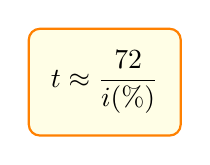
\begin{tikzpicture}
\node[rectangle, fill=yellow!10, rounded corners, inner sep=8pt, draw=orange, thick] (box) {
$\displaystyle t \approx \frac{72}{i(\%)}$
};
\end{tikzpicture}

Estimativa rápida do tempo para duplicar um capital:

\begin{itemize}
\item i = 1\% a.m. $\rightarrow$ t $\approx$ 72 meses
\item i = 2\% a.m. $\rightarrow$ t $\approx$ 36 meses
\item i = 6\% a.a. $\rightarrow$ t $\approx$ 12 anos
\item i = 12\% a.a. $\rightarrow$ t $\approx$ 6 anos
\end{itemize}

\section*{Exercícios Avançados}

\begin{enumerate}[leftmargin=*, start=9]

\item Análise de investimentos:
\begin{enumerate}[label=\alph*)]
\item Opção 1: CDB a 12\% a.a.
\item Opção 2: Poupança a 6\% a.a.
\item R\$ 10.000 por 5 anos. Diferença?
\end{enumerate}

\item Tempo de aplicação com logaritmos:
\begin{enumerate}[label=\alph*)]
\item Quanto tempo para R\$ 1000 virar R\$ 2000 a 5\% a.m.?
\item Se R\$ 5000 rendeu R\$ 1000 em 4 meses, qual a taxa mensal?
\item Em quanto tempo um capital quadruplica a 3\% a.m.?
\end{enumerate}

\item Problema de lógica:
\begin{enumerate}[label=\alph*)]
\item Um capital aplicado a juros compostos triplica em 5 anos.
  Em quanto tempo quadruplicaria?
\item Se a taxa é 2\% a.m., em quanto tempo o capital aumenta 50\%?
\end{enumerate}

\item Análise de gráfico:
\begin{center}
\begin{tikzpicture}[scale=0.7]
\draw[->] (0,0) -- (6,0) node[right] {Meses};
\draw[->] (0,0) -- (0,5) node[above] {Montante (R\$)};
\draw[red, thick] (0,2) -- (1,2.1) -- (2,2.205) -- (3,2.315) -- (4,2.431) -- (5,2.553);
\foreach \x in {0,1,2,3,4,5} \draw (\x,0.1) -- (\x,-0.1) node[below] {\x};
\end{tikzpicture}
\end{center}
\begin{enumerate}[label=\alph*)]
\item Qual o capital inicial?
\item Qual a taxa mensal aproximada?
\item Qual o montante após 10 meses?
\end{enumerate}

\end{enumerate}

\end{multicols}

\end{document}
